\begin{frame}[t,fragile]{重点的サンプリング}
  \begin{itemize}
    \setlength{\itemsep}{1em}
  \item 積分への寄与が大きな箇所をより重点的にサンプリング
    \[
    p(x) = e^{-x}
    \]
    \begin{tabular}{|c|c|c|}
      \hline
      $M$ & 平均値 & 誤差 \\
      \hline
      100 & 3.06 & 0.06 \\
      10000 & 3.142 & 0.006 \\
      1000000 & 3.1412 & 0.0006 \\
      \hline
    \end{tabular}
  \end{itemize}
  \vspace*{-7em}
  \hspace*{17em}
  \resizebox{!}{.45\textheight}{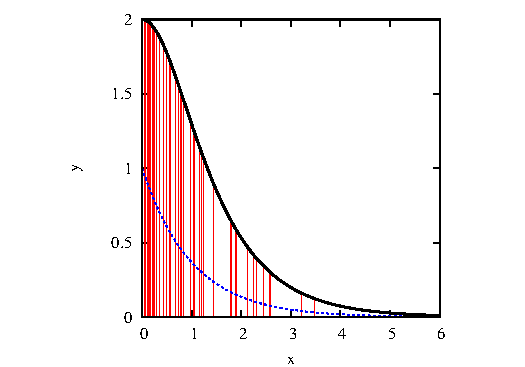
\includegraphics{image/coth-3.pdf}}
\end{frame}
